\part{Projektdokumentation}
Während der Durchführung des Projektes gab es verschiedenste Herausforderungen zu bewältigen und Entscheidungen zu treffen. Von der Organisation und Strukturierung der Gruppenarbeit, bis zur Wahl der Technologien, welche zur Realisierung des Projektes verwendet wurden. Dieses Kapitel beschreibt die Herangehensweisen des Teams und versucht reflektierend Schlüsse für zukünftige Projekte zu ziehen. 
\chapter{Anforderungs- und Problemanalyse}
\section{Methoden}
Aufgabe der Anforderungsanalyse in diesem Projekt war es herauszufinden
welches Problem die Kundin mit der zu entwickelnden Software lösen möchte. Dafür wurden
Interviews mit dem Kunden durchgeführt und entsprechende Ergebnisse mit Hilfe
von Audioaufzeichnung, Mitschriften und Fotografien protokolliert. Zur
detaillierten Beschreibung einzelner Abläufe des Systems wurden
Kreativtechniken wie das Zeichnen verschiedener Szenarien an einem Whiteboard
sowie die manuelle Simulation des Fahrstuhles mit einem aus Pappe gefertigten Modells durchgeführt.
\begin{figure}[hbt]
\centering
\subcaptionbox{Skizze der Fahrstuhlsimulation am Whiteboard}[0.49\linewidth]
{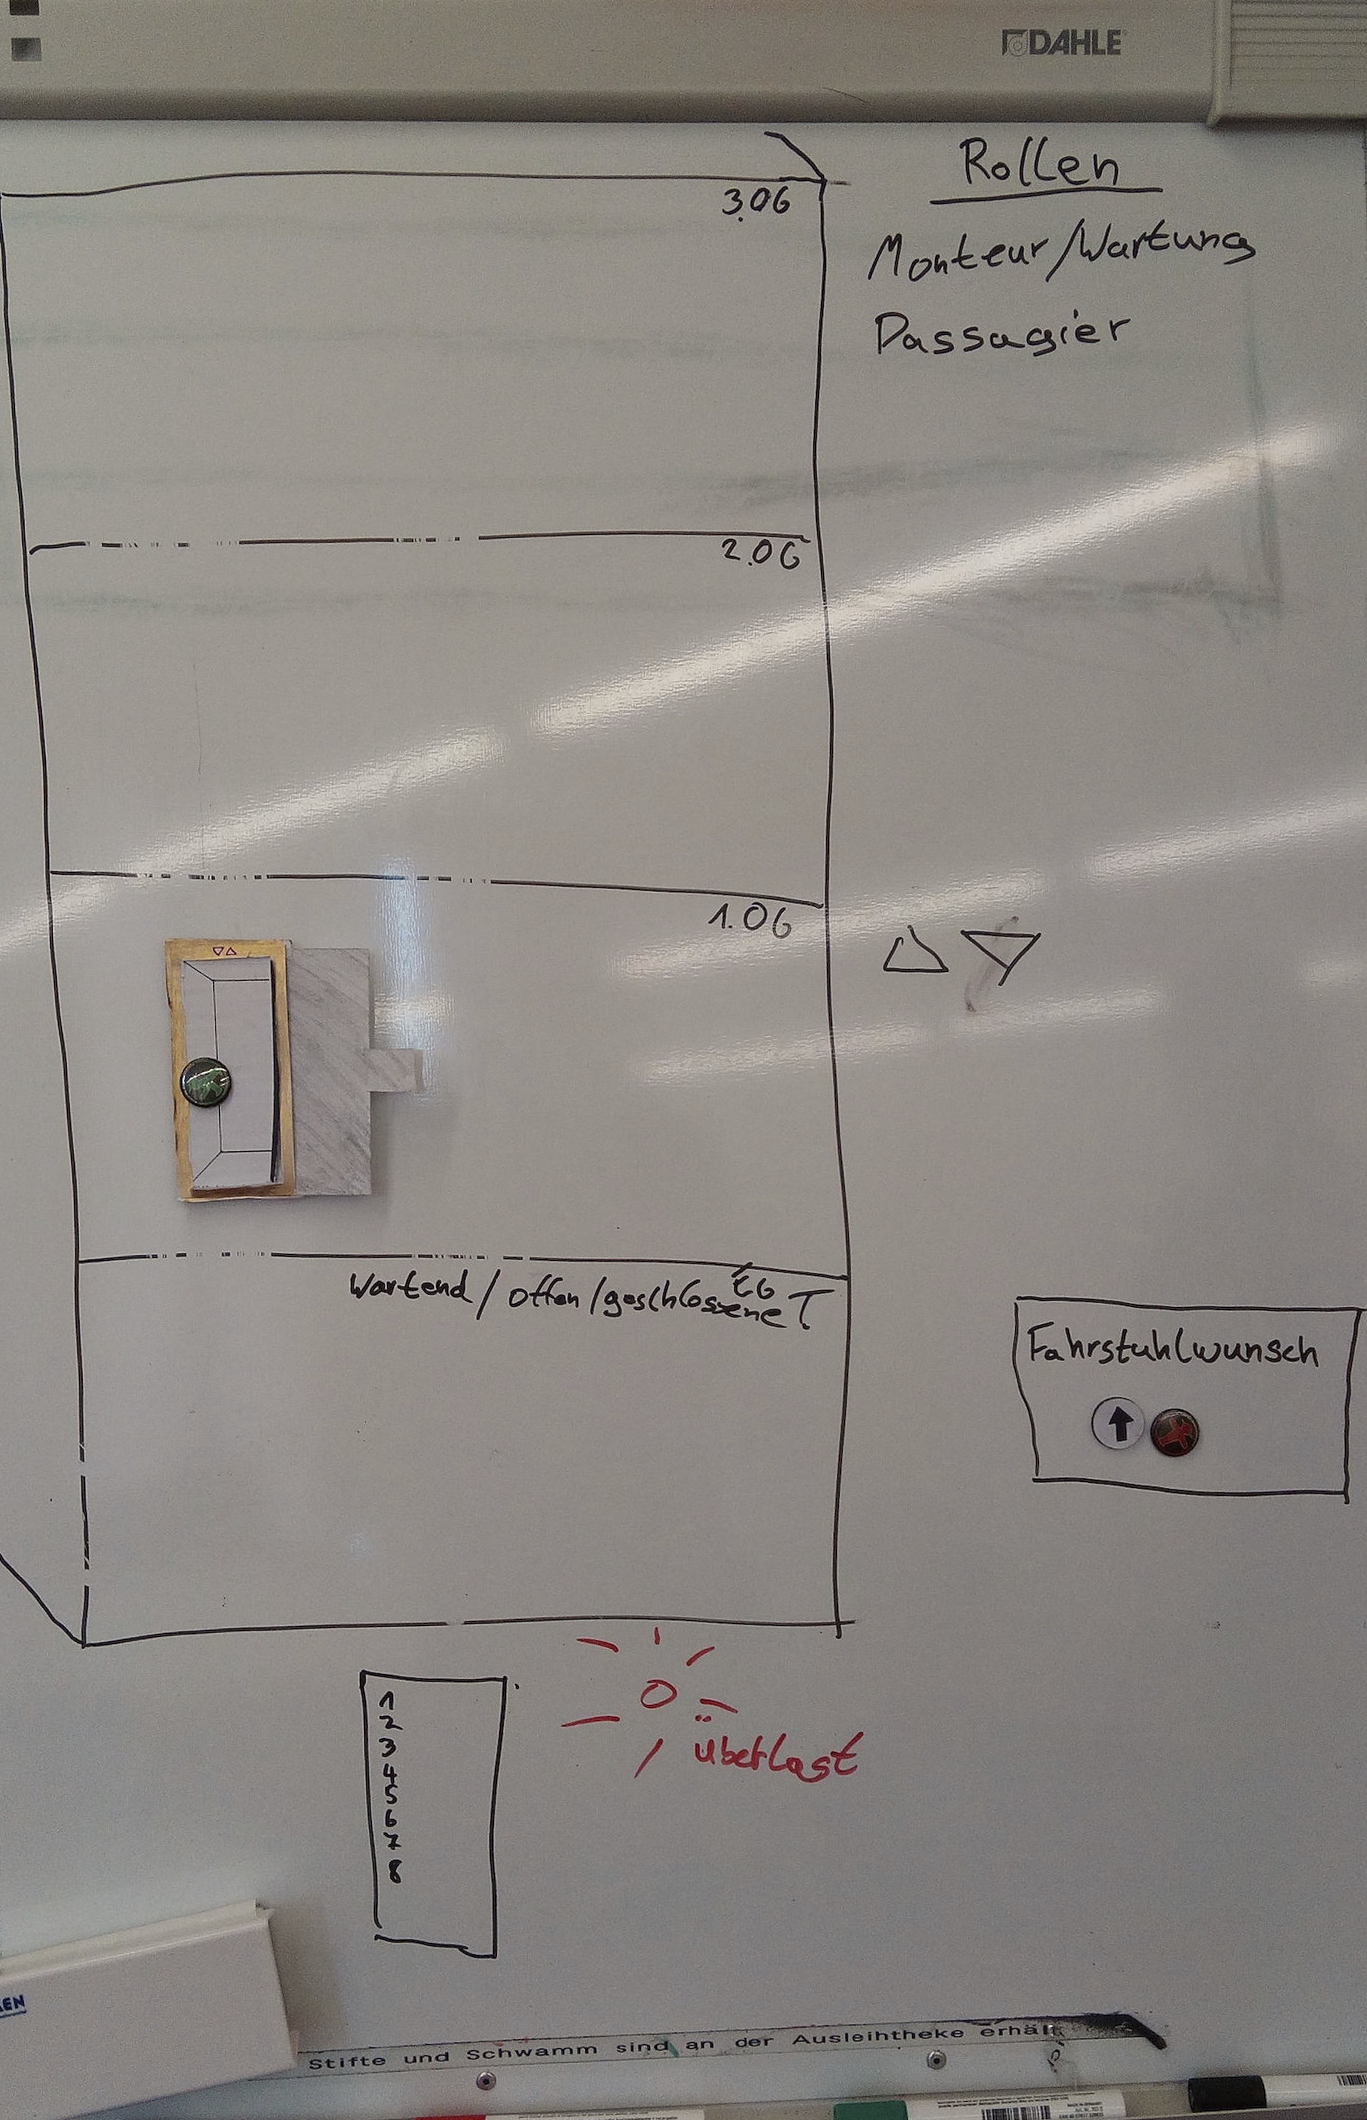
\includegraphics[height=8cm]{images/kundengespraech1.jpg}}
\subcaptionbox{Modell des Fahrstuhles}[0.49\linewidth]
{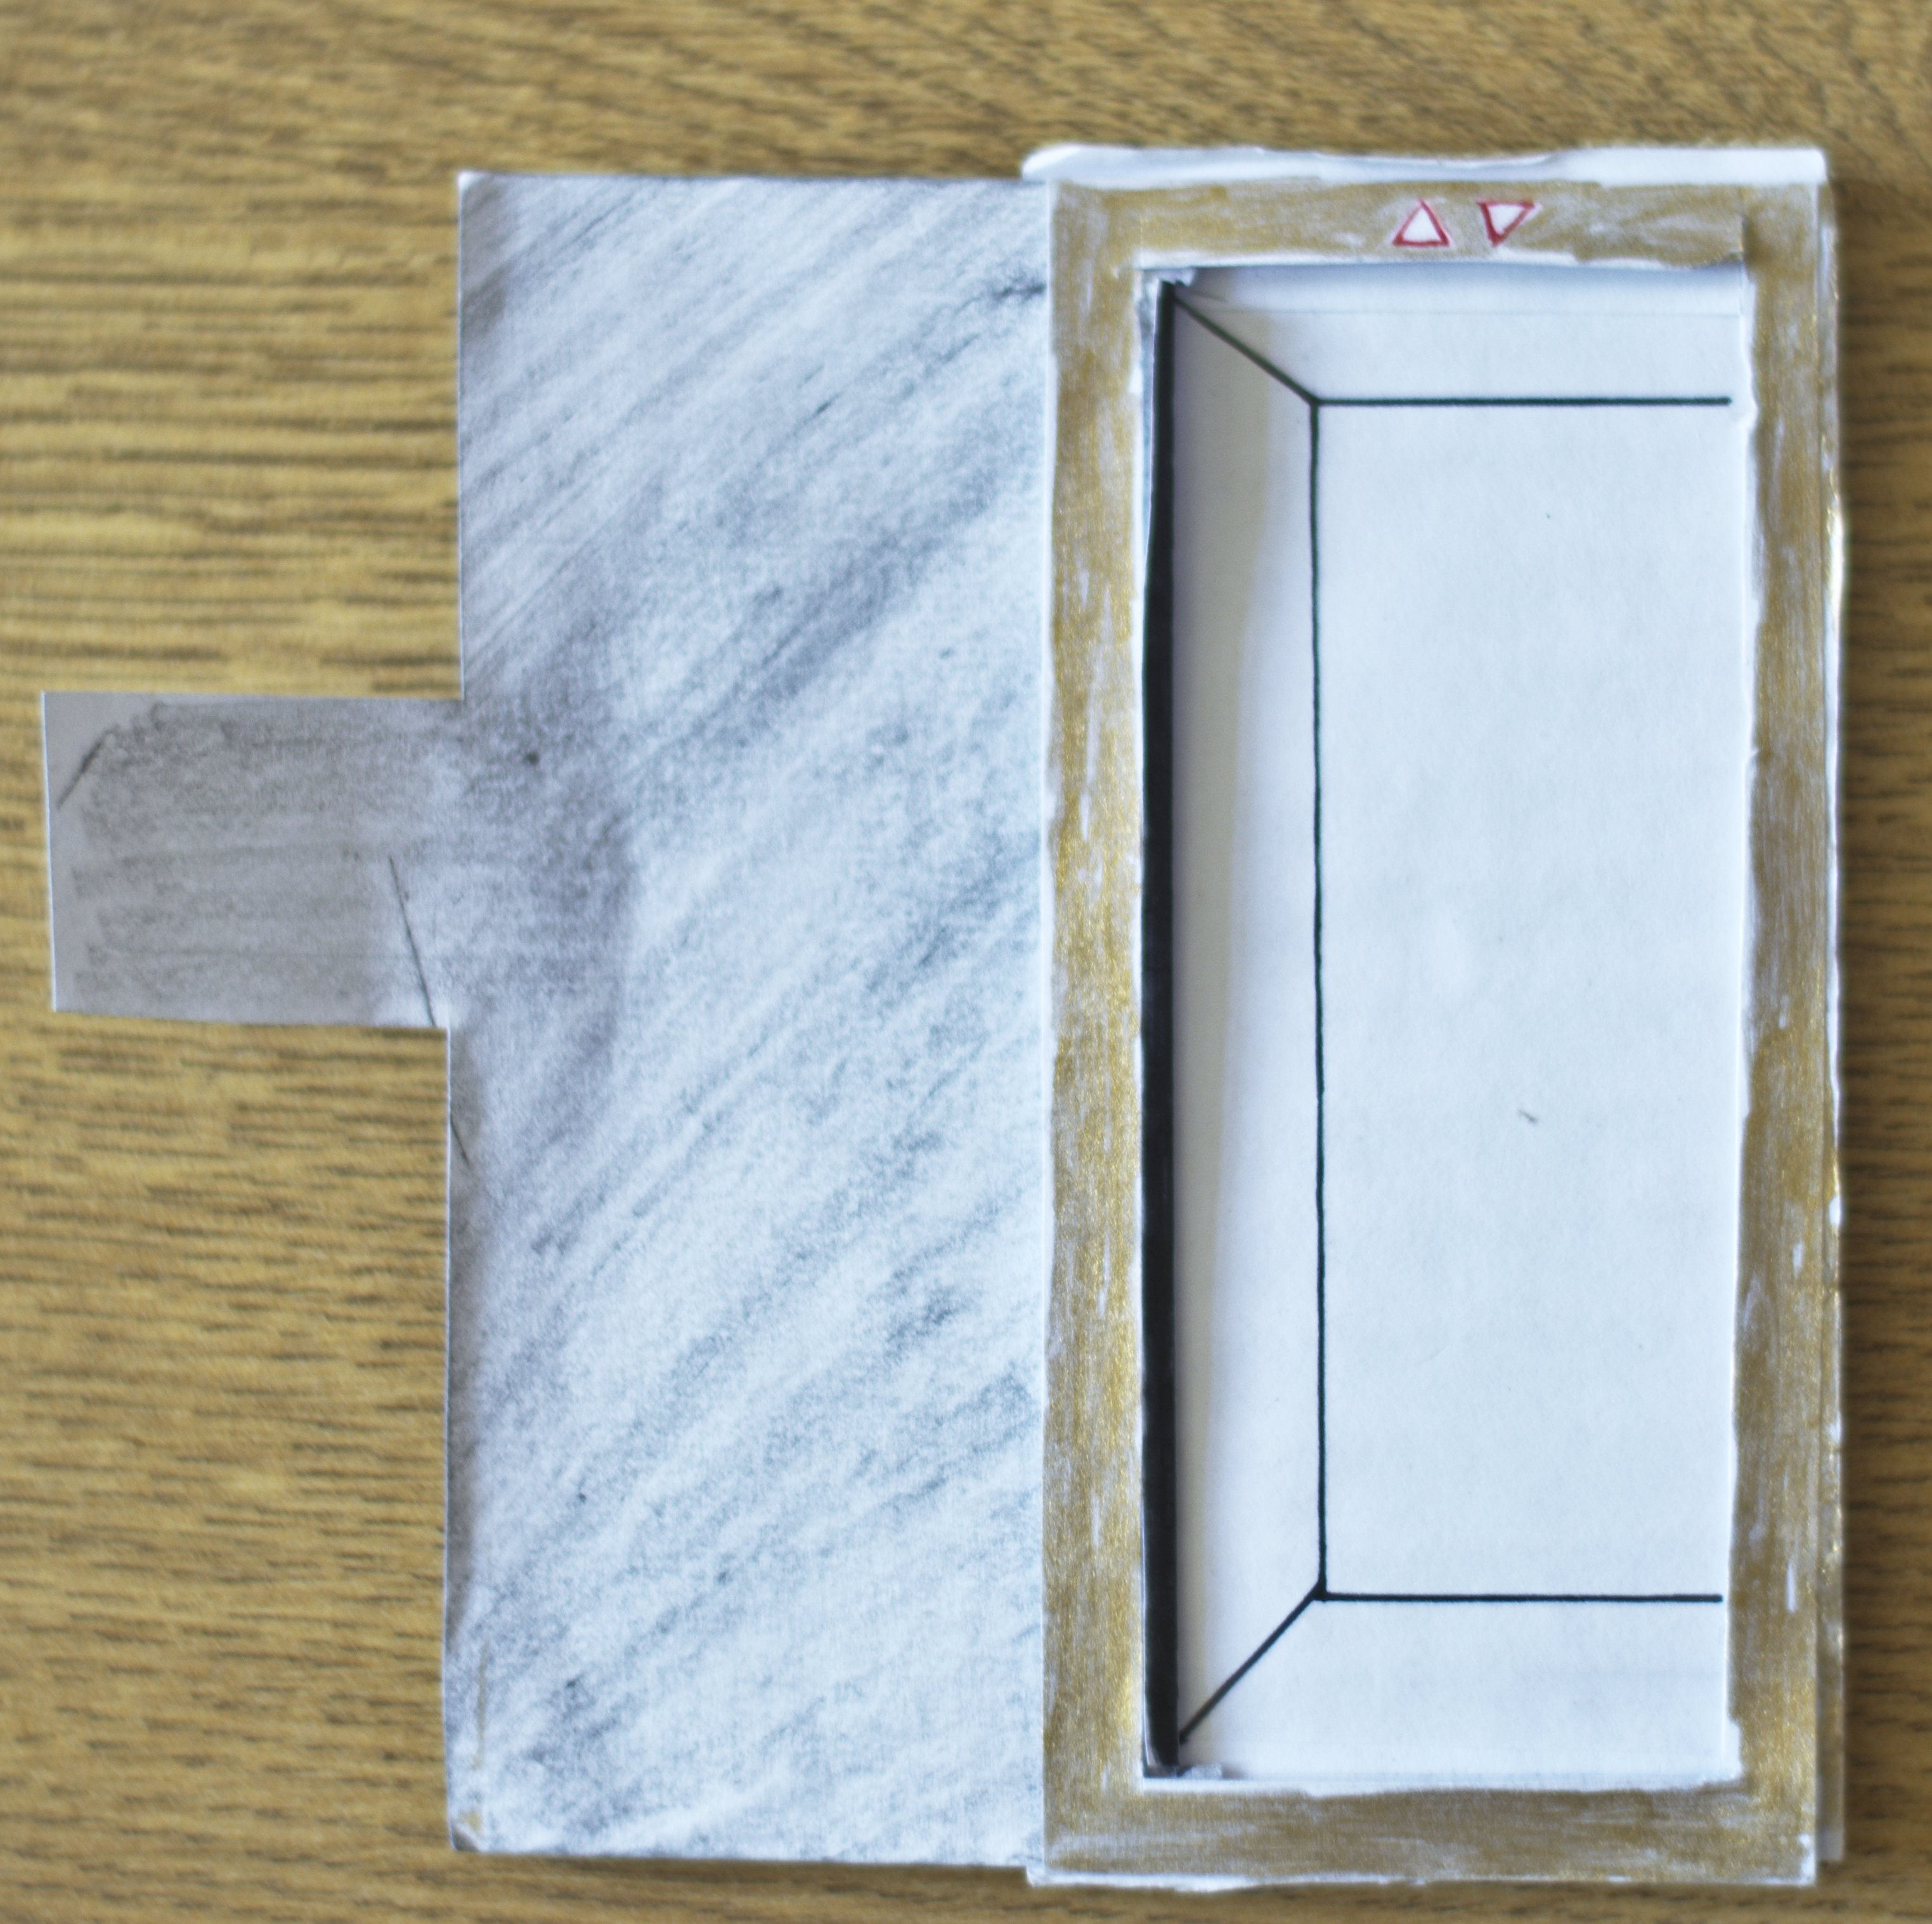
\includegraphics[height=8cm]{images/pappfahrstuhl.jpg}}
\caption{Kreativtechniken zur Anforderungsanalyse}
\end{figure}
Die folgenden grundlegende Fragen waren im Laufe der Analyse zu klären:
\begin{itemize}
	\item Wie viele Fahrstühle sollen verwendet werden können?
	\item Wie soll das Gebäude beschaffen sein?
	\item Welcher Algorithmus soll verwendet werden?
	\item Gibt es Schnittstellen zu anderen Systemen?
\end{itemize}
Weiterhin musste festgelegt werden ob die Priorität des Systems auf der
Simulation oder auf einer möglichst realitätsnahen Umsetzung eines Liftes liegt.
Im Laufe der Analyse und Modellierung entsprechender Anwendungsfälle
wurde ersichtlich, dass das System sich aus zwei Teilsystemen, der
\textbf{Fahrstuhlsteuerung} und der \textbf{Fahrstuhlsimulation} zusammensetzt,
deren Anforderungen getrennt voneinander beschrieben werden mussten.\\
Eine Besonderheit des Systems ist dabei die Umgebung in der es eingesetzt werden
soll, der Lehrbetrieb an einer Hochschule. Daraus ergaben sich spezielle
Anforderungen wie das Anzeigen der Zustandsübergänge die gesondert betrachtet
werden mussten.

\paragraph*{}Die Resultate der Analysephase, alle Anwendungsfälle und Vereinbarungen mit der Kundin wurden am Ende im Pflichtenheft festgehalten, welches als eigenständiges Dokument am Ende der Phase an die Kundin überreicht wurde. 
\section{Diagramme}
\subsubsection{Zustandsdiagramm}
Die wesentliche Funktionalität sowie der Algorithmus des Systems lassen sich in
dem Zustandsdiagramm abbilden. Um das bestmögliche Ergebnis zu erhalten haben
wir verschiedene Versionen des Diagramms entworfen und diese in Gruppentreffen diskutiert und überarbeitet.
\missingfigure[figwidth=\textwidth]{Zustandsdiagramm ggf. mehrere Versionen}


\chapter{Software-Entwurf}
Für die technische Umsetzung der Zustände in ausführbaren Quellcode ergaben sich folgende Entwurfsmuster:
\todo{Wir müssen aufpassen, dass wir eine klare Trennung zwischen Entwurfs-spezifischen Inhalten im Entwicklerhandbuch und hier vornehmen.}
\subsection*{State Design Pattern}
Vorteile, Nachteile, warum haben wir uns dageben entschieden?
\todo{Nachteile: großer Overhead, da hier nur 3 Zustände vorkommen, jedoch die Zustandsübergänge komplex sind}
\subsection*{Zustandstabelle}
\todo{nicht sinnvoll zwecks erweiterbarkeit/wartbarkeit}

Die eigentliche Herausforderung des Systems besteht nicht in den Zuständen, sondern in den Zustandsübergängen, da der Fahrstuhl bis auf wenige Ausnahmen wie von \textbf{Idle} nach \textbf{Stop} in jeden beliebigen Zustand springen kann.
\subsection*{Event Emitter}
\subsection{Observer Pattern}

\chapter{Qualitätssicherung}
\section{Umsetzung}
Zu Beginn des Projekts wurde beim der Erstellung des Pflichtenheftes auf saubere und eindeutige Formulierungen geachtet, da Probleme zu diesem Zeitpunkt die größten Auswirkungen auf die Qualität des Endprodukts besitzen.

\todo{Traceabillity hinzufügen -> jede Anforderung muss im Quellcode durch einen commit oder ähnlich nachverfolgbar sein}
\todo{Code Konventionen, statische Codeanalyse}

Für die automatischen Tests wurde das Testframework Jasmine\footnote{http://jasmine.github.io}

\section{Testfälle}


\chapter{Team-Organisation}
\section{Gruppenarbeit}
Um das Zusammenarbeiten in der Gruppe einfacher zu gestalten wurden verschiedene Technologien eingesetzt.
Zu finden von Terminen für Meetings wurde Doodle\footnote{\url{www.doodle.com}}  verwendet. Für die Kommunikation in der Gruppe Slack\footnote{\url{https://slack.com/}}.
\todo{Hier muss hin warum wir uns für JS und Co entschieden haben.}
\section{Verwendete Werkzeuge}
\section{Resümee}
